%\documentclass[12pt,twoside,abbrevs,bsc,logo,notimes,deptreport]{styles/cs4rep}
\documentclass[parskip]{styles/cs4rep}

% Packages
\usepackage{graphicx}
\usepackage{abbrevs}
\usepackage{acronym}
\usepackage{minted}
\usepackage{multirow}
\usepackage[backend=biber,sorting=none]{biblatex}
\usepackage{todonotes}
\usepackage{setspace}
\usepackage[breaklinks]{hyperref}

\addbibresource{refs/bibliography.bib}

\renewcommand\theFancyVerbLine{\normalsize\arabic{FancyVerbLine}}

\onehalfspacing

\begin{document}

% Project Details
\title{Crowdsourcing Usability Testing for Mobile Apps}
\author{Ben Kay}
\degree{Artificial Intelligence and Computer Science}
\project{4th Year Project Report}

%\submityear{2013}
%\graduationdate{June 2013}
\date{\today}

%\newacro{SQL}{Structured Query Language}
\newacro{ORM}{Object Relational Mapper}
\newacro{DBMS}{Database Management System}
\newacro{FUSE}{Filesystems in Userspace}
\newacro{GUI}{Graphical User Interface}
\newacro{NFS}{Network Filesystem}
\newacro{DSL}{Domain Specific Language}

\abstract{We directly and indirectly interact with thousands of databases per day. However, despite this widespread usage they are often hidden at the bottom of the software infrastructure and require bespoke solutions in order to allow users to interact with them.

One of the problems is that to interact with databases often requires domain knowledge of the database structure or query languages. There is a need for solutions that allow regular users to interact with databases. This project aims to be one such solution to the problem.}

% Extra Package Commands

%  \begin{preliminary}
    % Title Page
    \maketitle

    % Preamble
    \section*{Acknowledgements}

	I'd first like to thank my supervisor, Stratis Viglas, for keeping me on
	track and offering fantastic feedback throughout the year.

	I'd also like to thank Ewan Klein and the rest of my project group for
	offering a tenth pair of eyes on the progress of my project at our
	meetings.

	Finally I'd like to thank the numerous creators and maintainers of the
	\LaTeX\ \texttt{infthesis} class who stopped me procrastinating by doing
	much of the typesetting work beforehand.

%    \standarddeclaration
    %\dedication{

To Stephen McGruer for achieving the impossible and being angry for the entire
of 2011.

}
    \tableofcontents
%    \listoffigures
%  \end{preliminary}

  % Chapters 
  \chapter{Introduction}

Even though databases are used at the core of nearly all enterprise software,
most popular websites and many common desktop applications they are always
hidden behind layers of expensive, time consuming interface design and bespoke
software. Databases are avoided by even technical users, such as developers,
who will often not use them directly instead preferring to use technologies
such as \acp{ORM} (Hibernate, ActiveRecord, etc.) or alternate, more
user-friendly, query languages than \ac{SQL}.

\ac{SQL} is an complex language that is useful for lower level usage such as
debugging a particular query or the study of databases. Not helping this matter
are the many different dialects that each \ac{DBMS} imposes that the user
conforms to. This being one of the reasons that \acp{ORM} are used so widely.

\ac{SQL} is not suitable for non-technical users to perform any common tasks.
There is a need for tools that help all users easily interact with databases.
While there are already tools that provide a front end to help more technical
users manipulate them at a low level these tools require the user to understand
the difference between a table and a view or when to create an index in order
to maintain maximum performance from the database.

This is not acceptable in the general case. There should be a way of allowing
any user who is familiar with the basic usage of a computer to be able to
accomplish a good proportion of the tasks that the database can help with.

  \chapter{Background}

There are two distinct types of UI testing that can be performed when building
an application. One is ensuring the interface performs as according to the
specifications and does not crash unexpectedly, and the other is testing that
the interface as implemented according to the specifications is usable and
intuitive for a user. While the former type of testing can be harder and more
time consuming than testing units of code, it is still relatively easy to
automate - in the Android platform alone, there exist a number of existing
tools which can be used to accomplish this, for example the Robotium
\cite{robotium} framework, and monkey and monkeyrunner \cite{monkeyrunner}
applications that ship with the Android developer tools. Usability testing on
the other hand is not so simple, precisely because it is testing how
a \emph{human} reacts to the application compared to what is expected by the
application's developer. As such, most techniques rely on a human participant
or manual inspection of the interface.

\section{User (or Hallway) Testing}

The most common method of usability testing performed by application developers
is done by recruiting five or six participants who are unfamiliar with the
application being tested and chosen to cover the intended target audience as
widely as possible. It usually takes place in a controlled setting designed to
mimic, say, an office or living room, and the participant given tasks that are
intended to cover the use cases of an application. As an example, if
a calendar/organiser application were being tested then the participant might
be asked to ``enter a reminder about dinner out next friday''. While completing
the task they are told to think aloud about their reasoning behind the actions
taken, and how they expect the application to behave, hence it is known as
``Think Aloud'' testing. This method is based on work by K. A. Ericsson and H.
A. Simon \cite{ericsson1980verbal}, and gives information about how the
interface matches the participant's thinking, and highlights areas that need
improvement. An important part of using this technique is to ensure the
participants are not involved with the project in any way, otherwise they will
often already know how to accomplish the tasks given, missing ambiguities and
false paths.

\subsection{Remote Testing}

In the event that test participants cannot be located near to the test
location, videoconferencing and screen recording/webcam software can be
utilised to perform testing remotely. A few companies, such as
\url{usertesting.com} take advantage of this to offload the work of finding and
testing participants from the developer.  The cost of these services (at the
time of writing, from \$49 per participant for a mobile application), while
definitely worthwhile at key points of the development may be prohibitively
costly for a developer with a small budget to make use of often.

\section{Heuristic Evaluation}

Since there are many recognised common usability principles that apply to
software interfaces, an interface can be inspected by an expert reviewer and
judged as to how well it conforms to these principles (the ``heuristics'').
This method of testing is potentially cheaper than testing with actual users,
since it only requires one expert to perform (although better results may be
gained with more evaluators).  Due to this is can also be undertaken with
shorter notice and with greater frequency (depending on the availability of the
expert) than user testing.

Despite these advantages, heuristic evaluation cannot displace user testing
since the two methods do not catch all the same issues. In contrast, the two
methods are complementary, and can be used at different points in the
development process for maximal performance \cite{tan2009web, archer2010web}.

\subsection{Automated Methods}

As the principles and guidelines used when performing heuristic evaluation can
be formalised, tools that attempt to automatically evaluate applications are
available. The (desktop) web is the most active area for tools such as this,
for example USEFul \cite{dingli2011useful}, a program which automatically 
analyses websites, comparing them to a database of usability guidelines. Optimised
for desktop websites.

There are however no such services currently available for native Android apps,
making this approach useless for our use case, although tools for this purpose
could be developed in the future.

\section{A/B Testing}

One form of testing that is widely used, especially on the web, but equally
viable in mobile applications if the deployment mechanism allows it, to improve
usability. In this form of testing modifications are made to the interface
received by a random proportion of users, and success rate of a metric is
compared between the two versions. If the change gives a positive effect, then
it is incorporated into the version sent to all users. A/B testing is most effective
when the application is being used by a large number of users, such as a late
beta phase or when it is in production. It's not so suitable for the phases
of development before or during user testing or heuristic evaluation, and is
usually used to refine interfaces as opposed to making any large sweeping changes.

  \chapter{Formulation of the Problem}

The main obstacles to effective usability testing on the Android
platform are cost, expertise and the lack of effective automation.
If performing think aloud testing, participants must be found and
then travel to the site of the testing (or the developer travel to
them), and are usually paid for their time.  While there are services
that take care of much of the process on behalf of the developer,
the process tends to be costly, especially if it is done often.

Other types of usability testing such as heuristic evaluation must
be performed by experts to be effective.

Because of these obstacles, usability testing may not be performed
often or even at all during the development of a mobile application,
causing usability issues in the user interface to go undetected.

\todo{Keeping people engaged}

\section{Proposed Solution}

While analytics services can gather large amounts of data from the
interaction of users with an application, the lack of structure can
make it difficult to draw meaningful conclusions as information
about the intent of the user is lost when the data is gathered.
Without knowing the intent of users as they are using the application,
the data gathered cannot reveal where features of an application
are used or not used because their usability is poor, or whether
they are simply less popular.

Tasks which always have a specific structured workflow, such as a
checkout process, are easier to analyse with existing analytics
services, as user intent is clear. By giving the user more structured
tasks it should be possible to collect useful data from other parts
of a mobile application.

By combining some of the methodologies traditionally used in usability
testing with analytics, it should be possible to provide a structured
environment that can easily be given to people unfamiliar with an
application, and to easily gather data which will identify potential
problem areas with respect to usability.

The solution will take the form of a framework that can be easily
integrated into any mobile application, with as little modification
to the application's code as possible. The developer will define
tasks for the user to complete with defined starting points in the
app to make aggregation of data easier. Users can then attempt to
complete the tasks independently without there needing to be a
member of the development team present, as is usual with usability
testing, and the results will automatically be uploaded for the
developer to view at a later time. By aggregating the data from
many tests common problem areas should be able to be identified and
investigated further.

  \chapter{Design}

The core problem to solve is finding the best way to capture updates from
either the database or filesystem and present them on the other. There were two
main alternative approaches that could be taken in order to create a system
that would solve this problem.

The first approach is the most straightforward and requires a program to be
watching the database and filesystem for changes. Once a change is detected it
would then be mirrored by applying the corresponding changes in the opposite
system. For example, if a file was created on the filesystem a record would be
created in the database.

The second approach is more complicated than the first but implements a similar
idea. Instead of creating a program which monitors the standard filesystem for
changes we create a filesystem that can be mounted on the users system and
provides live updates of any changes through a system of callbacks.

An example of operations and their corresponding action in the other system is
shown in table \ref{tbl:mappings}.

\begin{table}
	\centering
	\begin{tabular}{|l|l|}
		\hline
		\textbf{Filesystem Action} & \textbf{Database Action} \\
		\hline
		Add a file & Create a record \\
		Remove a file & Delete a record \\
		Modify a file & Change a record \\
		Rename a directory & Rename a table \\
		\hline
	\end{tabular}
	\caption{Filesystem to/from Database Mappings}
	\label{tbl:mappings}
\end{table}

\section{Polling or Filesystem?}

\subsection{Polling}

The polling system, as outlined above, would be run at regular intervals to
give the illusion that both systems were directly linked. There are numerous
challenges with this implementation with the most prominent being detecting the
changes made on each side. Triggers that will execute when changes are made or
streaming logs of all changes can be used to monitor for changes in a database.
However, not all database management systems have support for these features.

Waiting for changes in a filesystem is possible simply by scanning over the
filesystem for any modification dates that have changed since the last scan was
performed. However, this syster is very ``brute force'' and may be slow on
systems with many files. To improve upon this method we may use operating
system APIs that allow us to register for callbacks when files are changed. The
libraries to perform these tasks are \texttt{inotify} for Linux and
\texttt{fs-events} for Mac OS X.

This is a less than ideal solution for checking for updates when we may have
millions of records and therefore millions files that need checking. This
solution just does not scale well even with the operating system assistance.
Additionally, the constant polling of the filesystem is a lot of wasted work
that will deplete the battery of laptops unnecessarily and waste power on
desktop machines. Instead, we should flip the problem around and instead of
looking for the files that have been changed, we should get any file that
changes to tell us about itself.

\subsection{Filesystem}

By using a filesystem instead of an separate polling program we tighten the
feedback loop from changes to the files to the database. By doing this we avoid
the potentially expensive operations of scanning the filesystem for changes and
have direct callbacks that reference the exact file changed. This has the
additional advantage of automatically handling migrating any changes back from
the database to the filesystem just by refreshing the current view.

% TODO: Add more stuff.

\section{Scaling Issues}

There is some concern about how this system scale up to the sizes that some
databases can and will reach. This is due to some unknowns as to how
a filesystem will perform once it has millions of files in it with each file
representing a record in the database. In order to mitigate this problem (if it
does exist) the files should be nested more deeply in a tree structure in order
to reduce the number of files in a directory down to reasonable levels.

Since users rightly demand that a filesystem is responsive at all times then
a non-functional requirement should be made that the database returns all
queries as quickly as reasonably possible. There are numerous ways that this
could be achieved such as the simple caching of values outside the database in
memory all the way up to using previous usage patterns to scan across the data
on the disk in order to load it into memory before the query is ever made and
creating useful indexes automatically to help regularly slow queries. However,
it is unwise to spend unnecessary time considering solutions to problems that
may not occur.

\section{The Querying Problem}
\label{sec:queryproblem}

A database has 4 main duties when it comes to presenting the user with data:
adding, updating, deleting, and updating. Our current solution to the problem
provides a good solution to adding, updating, and deleting records but querying
the database beyond basic operations is not easy to do with the limited actions
available to the filesystem. When querying or searching a filesystem, one would
normally use commands such as \texttt{find} or \texttt{grep}. These commands
take far too long to provide the desired results when presented with this many
files. Additionally, they are also not set up to use the information that
a database can provide when querying such as having ordering defined on
records.

In order to allow the user to perform more complex queries on the database
a separate application is needed. However it is critical that still presents
the database as a filesystem. If we look at how users perform complex sequences
of operations on a filesystem: there are two different approaches depending on
the level of expertise of the user.

\subsection{Mirroring Filesystem Solutions}

If we have a task that we would like to perform such as resizing all of the
images in a folder that were taken in the last week and which have the word
``flower'' in the filename then depending on the level of expertise of the user
they will probably approach this problem in two different ways.

A technical user will could write a shell script or use multiple commands
piped together to achieve the intended effect. A command such as the following
will perform the task shown in figure \ref{fig:shell}.

\begin{figure}[ht!]
  \centering
	\begin{verbatim}
	  find . -type f -name ".jpg" |
	    grep "flower" |
	    xargs convert -resize 50%
	\end{verbatim}
  \caption{Shell Workflow}
  \label{fig:shell}
\end{figure}

Instead of performing the action in one step the user splits up the command
into 3 logical steps of find the pictures, filter the ones with flower in the
name, and finally perform the resizing. There is a flow of data through the
series of commands that are used.

A non-technical user has a number of available operations to them. The most
widely used among Macintosh users is probably a program named \emph{Automator}
which is bundled with the operating system and integrates well with it. It
allows the user to create a similar workflow to shell scripts by composing
a sequence of similar duties to the programs above. An example of an
\emph{Automator} workflow is shown in figure~\ref{fig:automator}. This workflow
performs the same task as described above.

\begin{figure}[ht!]
  \centering
  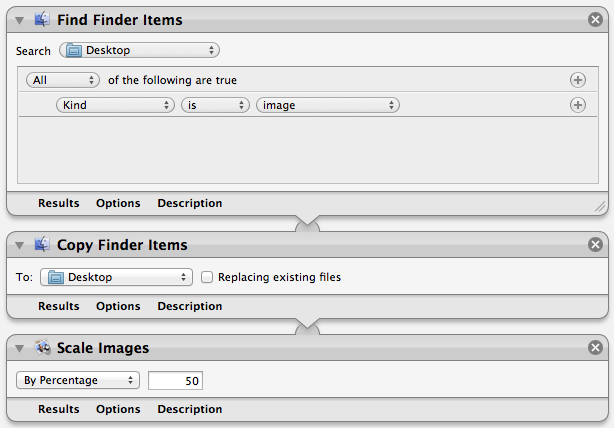
\includegraphics[width=0.9\textwidth]{images/automator}
  \caption{Automator Workflow}
  \label{fig:automator}
\end{figure}

We should be able to take this existing solution and paradigm and apply it to
the database querying problem. I believe that this will work especially well if
we make the records maintain their file-like qualities even inside the
application. In order to convert this graph of command into a database action
we are going to need to generate \ac{SQL} which will perform the desired
action. This is the next design challenge.

\subsection{Creating SQL}

The task of creating \ac{SQL} has been solved many different times when
creating \acp{ORM}. These often use Relational Algebra or something similar to
represent the compound operators before being converted to a sensible SQL
statement. Using a similar approach for this task would be sensible as it
mimics the graph structure that is described above. For example, a filter node
in the application above is equivalent to a selection wrapping everything above
it in the graph.

This intermediate relational algebra representation also has the advantage of
completing the metaphor above by replacing the more technical users requirement
of being able to drop down to a more direct interface to controlling the
database.

To this end I'm going to create an intermediate language that allows the user
to create complex \ac{SQL} queries by writing relational algebra in an
imperative style. This can then be combined with the filesystem by allowing
these files to be saved on it and having it return the results.

\subsection{Querying the Filesystem}

While more advanced users may be able to write the intermediate language
directly in order to query the database there needs to be a program to help
the majority of users to be able to use the system. The example used above
(\emph{Automator}) allows the users to create a simple flow of data through
different applications and services. We are able to see a similar pattern that
can be used to query databases by having the user create a flow that is
similar to the query graph that will be used inside the database.

The graph that the user creates can then be traversed in order to generate
the language described above.

TODO: More.

  \chapter{Implementation}

To allow easy integration into any Android app, the library is implemented
as an Android Library Project \cite{android-library}, which enables it to leverage the 
full functionality of the android platform - it can make use of its own assets and
layouts and manage its own dependencies - while being self contained and portable between 
projects. The only extra considerations that have to be made with this approach is to ensure
that all the project resources (layouts, strings, images etc.) are prefixed to avoid conflict
with the application the library is integrated into.

\section{Integrating the Library}

To specify tasks, the developer creates two json files which are
included in the application's \verb+assets/+ directory. These files specify all the tasks that are available to perform, and what order they will be performed in.

The testing functionality must be easy to remove/disable if the developer
does not want it present in the released version. To know when to begin and end tasks,
inject the library's user interface in the app, and gather data about the participant's 
performance, however, some integration with the application's code is needed.
To keep this to a minimum, all interaction with
the library in performed using the static \verb/Gamify/ class. This allows for
easy removal of the library as the developer can just find all references to
this class within the main application code and remove them. Since most Android
developers use \emph{Proguard} while compiling release versions, the rule below could be
included to automatically strip function calls to the library out of production versions.

\begin{minted}{text}
  -assumenosideeffects class com.example.Gamify {
    <methods>;
  }
\end{minted}

Alternatively, the library can also be disabled by passing \verb|false| when initialising. The
initialisation is done by calling \verb|init| in either the \verb|Application|
or initial \verb|Activity|'s \verb|onCreate| method, passing the two
aforementioned json files.

\begin{minted}{java}
  Gamify.init(this /* Context */, true /* Enabled */,
      "challenges.json", "sequences.json");
\end{minted}

\subsection{Defining tasks}

The ``challenges.json'' and ``sequences.json'' files define the tasks and
challenges that will be used in testing, identified by ids. Each task has a title, description, and optional instruction that appears at the top of the screen during a task, and defaults to the title. The sequences file defines groups of tasks, and which order they will be run in. It also specifies whether to reset the user's position in the application hierarchy after a task, or continue from where they finished the previous task.

\subsection{Integrating Tasks Into the Application}

To start a sequence,the developer can simply call a single method, specifying the ID of the sequence
to be started.

\begin{minted}{java}
  Gamify.startSequence("sequenceid");
\end{minted}

This will bring up the welcome screen and instructions as to how the testing works,
and allow the user to begin the first task in the sequence. Subsequent tasks are
automatically started when the previous one is finished.

Triggering points that will complete tasks are achieved with another method
call. For example if one task was completed by playing a song in the app, then
the corresponding code might look like:

\begin{minted}{java}
  public void playSong(Song song) {
    Gamify.completeChallenge("playsong");

    //... Code to play the song
  }
\end{minted}

If the ``playsong'' task is the current task, then it will be completed,
otherwise the method call will be ignored.

Beyond this, in each \verb|Activity|'s \verb|onResume| and \verb|onPause|
methods, the library must be notified.

\begin{minted}{java}
  @Override protected void onResume() {
     super.onResume();

     Gamify.onActivityResume(this);
  }

  @Override protected void onPause() {
     super.onPause();

     Gamify.onActivityPause(this);
  }
\end{minted}

This is so user interaction can be tracked, and the library's overlays can be
shown above the foreground activity. Since applications are usually designed so
that all activities inherit from a single base activity, this should not add
much extra overhead for the developer. These two methods can optionally be given 
additional arguments as strings, as in the case of the search activity in section
\ref{sec:developer-feedback}.

Finally, any additional navigation points can be tracked manually, by calling

\begin{minted}{java}
  Gamify.trackNavPoint("Navpoint name");
\end{minted}

This is useful for tracking fragment transactions, or anything else the tester
deems relevant.

\section{Developer Interface}

\subsection{Uploading and Storing Data}

Once a task has been completed or abandoned, the data must be collected and centralised.

To do this, the data is converted to a JSON format and automatically uploaded to a server
running a CouchDB database. A map-reduce query in the database ca be used to extract the data
in the form wanted for the graph display.

This approach was chosen for its simplicity, ease of implementation, and the ability to iterate quickly;
as CouchDB is a document oriented database, the raw JSON data can be stored as-is without the need
to define a schema or do any preprocessing. The map-reduce is run incrementally when new documents are 
received, and the results cached, so queries remain fast.

\subsection{Accessing Data}

A javascript application on a web page queries the database and generates the navigation graph for
each task. The query returns all the navigation paths recorded for a particular task, and the application
handles processing backtracks, merging the paths and rendering, using The Dracula Graph library \cite{dracula-graph} to display the final grahps.
  \chapter{Evaluation}

An important stage in developing a user interface (especially one which is
designed to improve usability) is to evaluate the system with user testing.
There are three reasons for performing this task: to check whether the software
actually helped the users, by how much the users were helped and also to see
how the software could be changed in order to improve its usability.

\section{Methods Used}

\subsection{User Testing}

The users were given a set of tasks to complete (section~\ref{sec:tasks}) and
a database schema that they should use to perform these tasks
(section~\ref{sec:schema}). The list of tasks was chosen in order to use as
many of the features of the application as possible. These tasks were then
performed on two different database querying applications: one that required
the user to enter \ac{SQL} and my application for querying the database.

The users were then timed on how long they took to complete the task (whether
they completed the task successfully or not). The time that it took to complete
the task along with whether or not the user was successful in completing the
task was then recorded. If the user made a small mistake with the \ac{SQL}
syntax or made a graph that did not provide the exact result then this was also
marked as a failure. During the user working through the tasks notes were taken
about any problems that the users had using the application.

\subsection{Questionnaire}

After completing the tasks described above the users filled in a short
questionnaire about their experience using both tools and the comparison
between them. The final section of the questionnaire asked the user for
longer-form answers about how they thought the application could be improved
and any other comments they had about using the application.

\section{Results Analysis}

\subsection{Minimal Previous SQL Experience}

For users who were new to SQL the system allowed the to query a database
effectively but admittedly at a much slower pace than users who were able to
call upon their \ac{SQL} experience. The best example of this is \textbf{User
1} who had no knowledge of SQL and yet was still able to use the application.

However, it was noted that a user who did not have at least a basic level of
understanding of \ac{SQL} had some trouble working out some of the phrases used
in in the application.

\begin{description}

\item[Select vs. Filter] \hfill

Some users found the distinction between \textbf{select} and \textbf{filter} (a
WHERE clause in \ac{SQL}) to be, in their mind, synonymous and often confused
the two.

\item[Equal vs. Matches] \hfill

User 1 in particular found the difference between \textbf{eq} ($=$) and
\textbf{matches} to be confusing.

\end{description}

Obviously, the times that the users who did not know \ac{SQL} took to complete
the task are in this case not useful as there is nothing to compare them to.
However, User 2 provided interesting data as they had a basic understanding of
\ac{SQL}. The time differences between the two were either insignificant or it
was found that using \ac{SQL} to query the database was considerably faster.

Where I feel the most interesting results come is that in all but one case that
if a user wasn't able to complete the task \emph{correctly} when using SQL then
they were able to create a valid and correct query using the graph query
application. This may show that even though users were slower at creating
queries using the application the queries that they created were syntactically
and semantically correct.

\subsection{Previous SQL Experience}

The users with previous \ac{SQL} experience provided the most complete and
useful timing results as they were able to provide results for both the
\ac{SQL} and new application questions. However, similar to \textbf{User 2}
their times were also similar or slower using the graph query application
rather than using plain \ac{SQL}.

The problems that the more advanced users encountered were more with the
usability of the program rather than any confusion with the usage of the
program itself. However, all users apart from \textbf{User 3} had difficulty
when they were required to join 3 tables together. The users who knew \ac{SQL}
were also able to create the simple (2 table equi-join) joins easily.

\subsection{Questionnaire Answers}

The most promising results by far were those from the questionnaire. Every
single user preferred using the graph query application to using \ac{SQL}.
Additionally, all of the users stated that they would consider using the
application to perform queries in the future.

\section{Improvements to the Application}

After getting feedback from the user testing there are a number of things that
I could do to improve the usability of the application and allow users that are
not familiar with \ac{SQL} to more easily use the application.

\begin{description}

\item[Remove Joins] \hfill

The idea of joins was confusing for all users. The more advanced users were
able to figure them out after some slight thought. The beginner users had
significant trouble understanding how they worked and how to apply them to the
problem. Both sets of users had trouble joining more than 2 tables together.

To this end it may be wise to remove the concept of joins from the application
entirely and automatically enter them into the queries if they are
needed.\footnote{TODO: Possibly cite Sasa's project work this year?} When
a user selects data that is sourced from more than 1 table we would
automatically scan the database for the list of tables that could be joined
together in order to compute the join. However, at the current moment the
application doesn't have a connection open to the database while it is running
it would be up to the user to enter in the schema details in order for this to
be computed. Alternatively we could allow the application to connect to the
database to gather the schema for itself.

The next problem is working out how to join two tables together also without
requiring the user to enter extra information. Given two tables there are a few
ways that we could compute the correct join attributes.

\begin{itemize}

\item Check for explicit foreign key definitions in the database.

\item Check to see for matching data types in the two tables.

\item Check to see if there are any clues in the names of the attributes. For
	example, \texttt{student\_id} will probably join to an attribute named
	\texttt{id} in a table named \texttt{student}.

\item Check to see if the values in one column of one table are in the other
	column of the other table.

\item All of the above. By using a compound score and weighting all of the
	different metrics based on how reliable they were we would be able to take
	the pairing with the maximum score and use that.

\end{itemize}

\item[Select/Filter Confusion] \hfill

Due to the confusion between the \textbf{select} and \textbf{filter} nodes and
their purposes there should be work done into clarifying the two. This could be
as simple as finding better names for them or alternatively removing the
concept of column selection completely and allowing the user select the columns
that they would like to get when they place the output node.

\item[Moving \& Deleting placed nodes] \hfill

Many users attempted to either move or delete nodes after they had been placed.
This is an obvious fix and just requires adding those features to the
application. This should also stop any user confusion at messy graphs after
they have placed the nodes in the wrong location.

\item[Arrows] \hfill

To help the users understand the flow of data through the application it may be
useful for them to visualise this by adding arrows on to the edges between
nodes. This makes sense as the graph is technically directed.

\end{description}

  \chapter{Conclusion}

Designing an intuitive user interface for a complex app will always be a
challenge, but for an app to survive in the competitive mobile
environment the developers must do their best to ensure this is the case.
While no alternative forms of testing can completely replace the lessons learnt
by working closely with users and observing their behaviour, strategies that
cut down on the amount of expensive and time consuming user testing needed
will always be welcome.

In this project I have demonstrated one such possible strategy, and shown 
that adapting existing techniques to a more automated, crowdsourced technology
can provide valuable insights into the way that people really interact with
an application. This way of testing should be cheaper, and possibly quicker, 
to perform, enabling usability testing to be integrated into the development
workflow in ways it could not be before. While there are definitely improvements that could be made,
and ideas that can be built upon - exploring data collection and presentation
possibilities alone could form the basis of another entire project - the library
as it is can already provide valuable feedback.
It could be used to enhance the rapid iteration of an interface, backing up new design decisions
almost immediately with real data, or help a small hobbyist developer
track down confusing or buggy areas of their app that previously went
completely unnoticed. Indeed it has already given the users of one app
a better experience, and I look forward to implementing the remainder
of the findings as soon as I possibly can.

  % Appendix
  \appendix

  \chapter{Evaluation} \label{apdx:evaluation}

\section{Challenges}

\begin{minted}{javascript} 
[

  {
    id: "connect", 
    title: "Getting started",
    description: "Get connected to the browser you've set up.",
    instruction: "Connect to a browser."
  },

  {
    id: "playlibrary",
    title: "Play your collection.",
    description: "Now we're connected, it would be nice to get some music
        playing. Try playing all the songs in your collection."
  },
  
  {
    id: "skipsong",
    title: "Skip to the next song.",
    description:"Let's pretend you're bored of this one. Skip to the next
        song."
  },
  
  {
    id: "startshuffle",
    title: "Turn on shuffle.",
    description:"How about mixing things up a bit? Try turning on shuffle."
  },
  
  {
    id: "search",
    title: "Searching for music.",
    description: "Search for and play the song \"Shuffle\" by Bombay Bicycle
        Club",
    instruction: "Play \"Shuffle\" by Bombay Bicycle Club"
  },
  
  {
    id: "viewalbum",
    title: "Viewing an album",
    description: "There's a song called \"Eyesdown\" by Bonobo in your
        favourites, and you want to check out the rest of the album.",
    instruction: "Open the album for Eyesdown."
  },
  
  {
    id: "addalbumtoplaylist",
    title: "Add something to a playlist",
    description: "You decide that you like the whole album, and want to
        save it in a playlist.",
    instruction: "Add all of \"Black Sands\" to a playlist."
  }

] 
\end{minted}


  % Bibliography
  \printbibliography
  
\end{document}
